\chapter{Application requirements and specifications}
\label{chap:specs}

\par The main goal of the application is to create an alternative way of interacting with a live video. For this purpose a deep learning neural network is used, more precisely a MobileNet model pretrained on the ImageNet dataset, with custom final layers for identification. The machine learning algorithm will identify hand gestures, acting as the controlling tools for the application. 

\section{Application requirements}
\label{sec:specssec1}

\par The main focus of the application is the alternative way of interacting with the live video feed, providing feature for drawing with a finger, using simple hand gestures for clearing the drawings, for zooming in on a specific section of the video, for changing the volume of the recording and for taking a screenshot.
\par Besides the hand driven way of interactions the volume settings and the screenshot features all have a specific buttons and toggles, so they can be worked with normally with normal mouse actions.
\par The application can also be used as a simple video recording software, providing settings options for camera and microphone selection, changing the folder to which save the video files and screenshots.
\par All of the above is in visual format in the use case diagram below \ref{fig:usecase}, which was created by an online tool called Lucidchart \cite{lucidchart}.

\begin{figure}
    \centering
    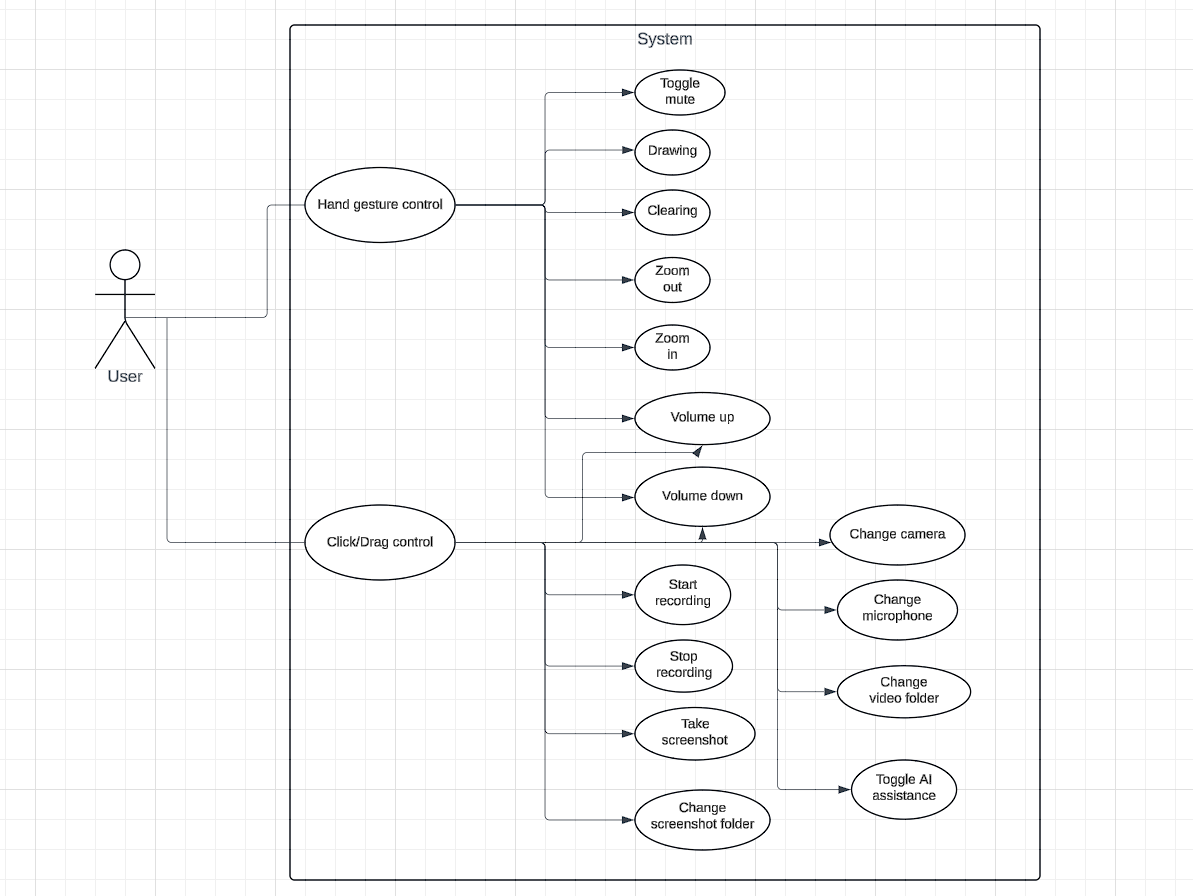
\includegraphics[width=0.8\linewidth]{figures/UseCaseDiagram.png}
    \caption{Use case diagram for the functionalities of the application}
    \label{fig:usecase}
\end{figure}

\subsection{Functional requirements}
\label{sec:specssec1subsec1}

\par To see the functionalities of the applications in an easier way, all of the above mentioned features are represented and described as use cases. The list with them is presented in Table\ref{UseCaseTable}, while the descriptions will be in the ones after.

\begin{table}[htbp]
\begin{center}
\begin{tabular}
{|p{90pt}|p{270pt}|}
\hline
 Use Case & Name\\
\hline 
\hline F1 & Start recording \\
\hline F2 & Stop recording \\
\hline F3 & Take screenshot \\
\hline F4 & Change volume up \\
\hline F5 & Change volume down \\
\hline F6 & Change video folder path \\
\hline F7 & Change screenshot folder path \\
\hline F8 & Change camera used during recording \\
\hline F9 & Change microphone used during recording \\
\hline F10 & Toggle artificial intelligence assistance \\
\hline F11 & Draw during recording \\
\hline F12 & Clear screen after drawing \\
\hline F13 & Toggle being muted \\
\hline F14 & Zoom in a portion of the video \\
\hline F15 & Zoom out \\
\hline
\end{tabular}
\end{center}
\caption{The application's functionalities represented as use cases}
\label{UseCaseTable}
\end{table}

\subsection{Functional requirements descriptions}
\label{sec:specssec1subsec1d1}

\par The F1 requirement is responsible for starting the video capture process. The steps and requirements for this functionality can be found in the table below \ref{F1Table}.
\par Prerequisites: The user chose a functioning camera and microphone; The user chose a path for the video to be saved in.
\par Post: The live feed of the video recording shows up on the screen; A pop-up error message is shown that the start was not successful.

\begin{table}[htbp]
\begin{center}
\begin{tabular}
{|p{180pt}|p{180pt}|}
\hline
 User & System\\
\hline 
\hline 1. The user presses the Start button &  \\
\hline  & 2. The system checks for a functioning camera and microphone \\
\hline  & 3. The system checks if the folder path given exists or not \\
\hline  & 4 The system starts the video capture \\
\hline  & 4.1 The system presents the live feed on the screen \\
\hline  & 4.2 The system shows a pop-up error message about the failure \\
\hline
\end{tabular}
\end{center}
\caption{F1 Functionality steps}
\label{F1Table}
\end{table}

\par The F2 requirement is responsible for stopping the video capture process. The steps and requirements for this functionality can be found in the table below \ref{F2Table}.
\par Prerequisites: The video recording is running successfully.
\par Post: The live feed on the screen will stop and turn into a black image and the video is present in the chosen folder; A pop-up message is shown about the failure of stopping the capturing.

\begin{table}[htbp]
\begin{center}
\begin{tabular}
{|p{180pt}|p{180pt}|}
\hline
 User & System\\
\hline 
\hline 1. The user presses the Stop button &  \\
\hline  & 2. The system stops the recording process \\
\hline  & 3. The system creates the final video file in the selected folder \\
\hline  & 3.1 A black image is shown instead of the live feed \\
\hline  & 3.2 The system shows a pop-up error message about the failure \\
\hline
\end{tabular}
\end{center}
\caption{F2 Functionality steps}
\label{F2Table}
\end{table}

\par The F3 requirement is responsible for taking a screenshot from the live feed. The steps and requirements for this functionality can be found in the table below \ref{F3Table}.
\par Prerequisites: The video recording is running successfully; A valid path is chosen as the screenshot folder.
\par Post: A pop-up message shows the screenshot was successfully taken and the picture will be present in the given folder; A pop-up error message is shown.

\begin{table}[htbp]
\begin{center}
\begin{tabular}
{|p{180pt}|p{180pt}|}
\hline
 User & System\\
\hline 
\hline 1. The user presses the Screenshot button &  \\
\hline  & 2. The system saves the last frame as an image in the chosen folder \\
\hline  & 3.1 A pop-up message is shown that the screenshot was taken successfully \\
\hline  & 3.2 The system shows a pop-up error message about the failure \\
\hline
\end{tabular}
\end{center}
\caption{F3 Functionality steps}
\label{F3Table}
\end{table}

\par The F4 requirement is responsible for changing the volume up. The steps and requirements for this functionality can be found in the table below \ref{F4Table}.
\par Prerequisites: The volume is not at 100 percent; For hand gesture control the recording is running and the AI assistance is turned on.
\par Post: The volume of the audio will be changed in the current or next recording.

\begin{table}[htbp]
\begin{center}
\begin{tabular}
{|p{180pt}|p{180pt}|}
\hline
 User & System\\
\hline 
\hline 1.1 The user moves the volume slider to the right &  \\
\hline 1.2 The user show a specific hand gesture &  \\
\hline  & 2. The system saves the volume modifier accordingly \\
\hline
\end{tabular}
\end{center}
\caption{F4 Functionality steps}
\label{F4Table}
\end{table}

\par The F5 requirement is responsible for changing the volume down. The steps and requirements for this functionality can be found in the table below \ref{F5Table}.
\par Prerequisites: The volume is not at 0 percent;For hand gesture control the recording is running and the AI assistance is turned on.
\par Post: The volume of the audio will be changed in the current or next recording.

\begin{table}[htbp]
\begin{center}
\begin{tabular}
{|p{180pt}|p{180pt}|}
\hline
 User & System\\
\hline 
\hline 1.1 The user moves the volume slider to the left &  \\
\hline 1.2 The user show a specific hand gesture &  \\
\hline  & 2. The system saves the volume modifier accordingly \\
\hline
\end{tabular}
\end{center}
\caption{F5 Functionality steps}
\label{F5Table}
\end{table}

\par The F6 requirement is responsible for changing the folder path for the video files. The steps and requirements for this functionality can be found in the table below \ref{F6Table}.
\par Prerequisites: The video recording is not running.
\par Post: The folder path for the video files will be changed accordingly and the user is sent back to the main window.

\begin{table}[htbp]
\begin{center}
\begin{tabular}
{|p{180pt}|p{180pt}|}
\hline
 User & System\\
\hline 
\hline 1. The user presses the Settings button &  \\
\hline  & 2. The current window is changed to the Settings window \\
\hline 3. The user presses the "Choose Path" button in the "Video folder path" section&  \\
\hline  & 4. The windows File explorer opens \\
\hline 5. The user chooses a folder &  \\
\hline  & 6. The system changes the path to the chosen one without saving it \\
\hline 7. The user presses the Save button &  \\
\hline  & 8. The system saves the setting changes to the configuration file \\
\hline  & 9. The system switches back to the main window \\
\hline
\end{tabular}
\end{center}
\caption{F6 Functionality steps}
\label{F6Table}
\end{table}

\par The F7 requirement is responsible for changing the folder path for the screenshots. The steps and requirements for this functionality can be found in the table below \ref{F7Table}.
\par Prerequisites: The video recording is not running.
\par Post: The folder path for the screenshots will be changed accordingly and the user is sent back to the main window.

\begin{table}[htbp]
\begin{center}
\begin{tabular}
{|p{180pt}|p{180pt}|}
\hline
 User & System\\
\hline 
\hline 1. The user presses the Settings button &  \\
\hline  & 2. The current window is changed to the Settings window \\
\hline 3. The user presses the "Choose Path" button in the "Screenshot folder path" section&  \\
\hline  & 4. The windows File explorer opens \\
\hline 5. The user chooses a folder &  \\
\hline  & 6. The system changes the path to the chosen one without saving it \\
\hline 7. The user presses the Save button &  \\
\hline  & 8. The system saves the setting changes to the configuration file \\
\hline  & 9. The system switches back to the main window \\
\hline
\end{tabular}
\end{center}
\caption{F7 Functionality steps}
\label{F7Table}
\end{table}

\par The F8 requirement is responsible for changing the used camera. The steps and requirements for this functionality can be found in the table below \ref{F8Table}.
\par Prerequisites: The video recording is not running.
\par Post: The chosen camera to be in use will be changed and the user is sent back to the main window.

\begin{table}[htbp]
\begin{center}
\begin{tabular}
{|p{180pt}|p{180pt}|}
\hline
 User & System\\
\hline 
\hline 1. The user presses the Settings button &  \\
\hline  & 2. The current window is changed to the Settings window \\
\hline 3. The user presses the drop-down list in the Camera section&  \\
\hline  & 4. The systems shows a list of available cameras \\
\hline 5. The user chooses a camera from the list &  \\
\hline  & 6. The system changes the camera to the chosen one without saving it \\
\hline 7. The user presses the Save button &  \\
\hline  & 8. The system saves the setting changes to the configuration file \\
\hline  & 9. The system switches back to the main window \\
\hline
\end{tabular}
\end{center}
\caption{F8 Functionality steps}
\label{F8Table}
\end{table}

\par The F9 requirement is responsible for changing the used microphone. The steps and requirements for this functionality can be found in the table below \ref{F9Table}.
\par Prerequisites: The video recording is not running.
\par Post: The chosen microphone to be in use will be changed and the user is sent back to the main window.

\begin{table}[htbp]
\begin{center}
\begin{tabular}
{|p{180pt}|p{180pt}|}
\hline
 User & System\\
\hline 
\hline 1. The user presses the Settings button &  \\
\hline  & 2. The current window is changed to the Settings window \\
\hline 3. The user presses the drop-down list in the Microphone section&  \\
\hline  & 4. The systems shows a list of available microphones \\
\hline 5. The user chooses a microphone from the list &  \\
\hline  & 6. The system changes the microphone to the chosen one without saving it \\
\hline 7. The user presses the Save button &  \\
\hline  & 8. The system saves the setting changes to the configuration file \\
\hline  & 9. The system switches back to the main window \\
\hline
\end{tabular}
\end{center}
\caption{F9 Functionality steps}
\label{F9Table}
\end{table}

\par The F10 requirement is responsible for toggling the AI assistance during video recording. The steps and requirements for this functionality can be found in the table below \ref{F10Table}.
\par Prerequisites: The video recording is not running.
\par Post: The AI assistance will be toggled on or off and the user is sent back to the main window.

\begin{table}[htbp]
\begin{center}
\begin{tabular}
{|p{180pt}|p{180pt}|}
\hline
 User & System\\
\hline 
\hline 1. The user presses the Settings button &  \\
\hline  & 2. The current window is changed to the Settings window \\
\hline 3. The user presses the toggle button in the "AI assistance" section  to change status&  \\
\hline  & 4. The system toggles the service on or off without saving the change \\
\hline 5. The user presses the Save button &  \\
\hline  & 6. The system saves the setting changes to the configuration file \\
\hline  & 7. The system switches back to the main window \\
\hline
\end{tabular}
\end{center}
\caption{F10 Functionality steps}
\label{F10Table}
\end{table}

\par The F11 requirement is responsible for hand driven drawing during video recording. The steps and requirements for this functionality can be found in the table below \ref{F11Table}.
\par Prerequisites: The video recording is running and the AI assistance is turned on.
\par Post: Given a specific hand gesture the system draws on the video feed following the users finger, visible both on the live feed and in the recording.

\begin{table}[htbp]
\begin{center}
\begin{tabular}
{|p{180pt}|p{180pt}|}
\hline
 User & System\\
\hline 
\hline 1. The user shows a specific hand gesture on the camera &  \\
\hline  & 2. The system whitens the pixels in a small radius near the finger of the user \\
\hline
\end{tabular}
\end{center}
\caption{F11 Functionality steps}
\label{F11Table}
\end{table}

\par The F12 requirement is responsible for clearing the video feed of any drawing during recording. The steps and requirements for this functionality can be found in the table below \ref{F12Table}.
\par Prerequisites: The video recording is running and the AI assistance is turned on.
\par Post: Given a specific hand gesture the system clears the video feed of any drawing.

\begin{table}[htbp]
\begin{center}
\begin{tabular}
{|p{180pt}|p{180pt}|}
\hline
 User & System\\
\hline 
\hline 1. The user shows a specific hand gesture on the camera &  \\
\hline  & 2. The system clears the video feed of any hand drawing \\
\hline
\end{tabular}
\end{center}
\caption{F12 Functionality steps}
\label{F12Table}
\end{table}

\par The F13 requirement is responsible for toggling being muted via hand gesture during video recording. The steps and requirements for this functionality can be found in the table below \ref{F13Table}.
\par Prerequisites: The video recording is running and the AI assistance is turned on.
\par Post: Given a specific hand gesture the system toggles between being muted and the previous audio level.

\begin{table}[htbp]
\begin{center}
\begin{tabular}
{|p{180pt}|p{180pt}|}
\hline
 User & System\\
\hline 
\hline 1. The user shows a specific hand gesture on the camera &  \\
\hline  & 2. The system toggles between being muted, audio level 0 percent and the previous level before the mute \\
\hline
\end{tabular}
\end{center}
\caption{F13 Functionality steps}
\label{F13Table}
\end{table}

\par The F14 requirement is responsible for zooming in a portion of the video controlled by a hand gesture. The steps and requirements for this functionality can be found in the table below \ref{F14Table}.
\par Prerequisites: The video recording is running and the AI assistance is turned on; The video feed is not zoomed in.
\par Post: Given a specific hand gesture the system zooms in a portion of the video where the users hand is.

\begin{table}[htbp]
\begin{center}
\begin{tabular}
{|p{180pt}|p{180pt}|}
\hline
 User & System\\
\hline 
\hline 1. The user shows a specific hand gesture on the camera &  \\
\hline  & 2. The system zooms in to the portion of the video where the users hand is present \\
\hline
\end{tabular}
\end{center}
\caption{F14 Functionality steps}
\label{F14Table}
\end{table}

\par The F15 requirement is responsible for zooming out of the zoomed in video feed. The steps and requirements for this functionality can be found in the table below \ref{F15Table}.
\par Prerequisites: The video recording is running and the AI assistance is turned on; The video feed is already zoomed in.
\par Post: Given a specific hand gesture the system zooms out, showing the full video.

\begin{table}[htbp]
\begin{center}
\begin{tabular}
{|p{180pt}|p{180pt}|}
\hline
 User & System\\
\hline 
\hline 1. The user shows a specific hand gesture on the camera in the zoomed in portion of the video &  \\
\hline  & 2. The system zooms out, showing the full video feed \\
\hline
\end{tabular}
\end{center}
\caption{F15 Functionality steps}
\label{F15Table}
\end{table}

\subsection{Non-functional requirements}
\label{sec:specssec1subsec2}

\par The application only has one version for the windows operating system, the results of running it on Linux, MacOS or any other operating system is undefined, they have not been test.
\par The processing of the input images from the video feed is done in real-time with the frame rate being determined by the input camera. The hand gesture identification and finger tracking is done on every second or third frame, depending on frame rate of the recording in the current moment.
\par The saving of the video files and images are done by only accessing those particular folders, with a naming convention of Recording\\Screenshot with the current date and time, so conflicts with other existing files is almost impossible, at the very least highly unlikely.

\subsection{System requirements}
\label{sec:specssec1subsec3}

\par The application only runs Windows operating system, needing the Windows 10 or 11 64-bit version, running on other versions may result in undefined behaviour.
\par In terms of the CPU the application was tested on Ryzen 7 4800h with a clock speed of 2.9 Gigahertz, from which 20-25 percent was used while running. From this data, an assumption can be drawn that as a baseline, a hardware similar to an intel core i7-9750h with a clock speed of 2.6 Gigahertz is advised. By having a weaker CPU the application may run into lagging issues when it comes to the rel-time performance of image processing.
\par The RAM used by the application is relatively small, using only 300 megabytes from a 3200 Megahertz unit.
\par In terms of storage, the application only needs around 300 Megabytes. The real impact will come from the saved video and screenshot files, depending on the file type in which they are saved.
\par To be able to use the application, the user also needs a working camera and a working microphone.

\label{sec:specssec2}

\section{Technical specifications}
\label{sec:specssec2}

\par For the purpose of easier integration of the deep learning model, the language used to develop the application is python, since most frameworks used for machine learning are written in this.
\par For creating and working with the MobileNet architecture, I use the TensorFlow \cite{tensorflow2015-whitepaper} and Keras framework \cite{chollet2015keras}. TensorFlow is an open-source project developed by Google giving an easy API for developing machine learning models efficiently, by wrapping up the more complex C++ and CUDA core functionalities. It also supports Keras, which is an open-source neural network library, providing an easy interface for building and teaching models, while also containing several known once, so they can be accessed with ease.
\par For the video capturing and the opencv library \cite{opencv_library}, which is open-source computer vision library written in mostly C++ and it is often used in machine learning projects. Because of that reason, the data, which is given back is easy to process and use in different models, making the development process that much easier.
\par Since the opencv library used for the capturing the visuals does not record audio as well, I use the pyaudio library, designed to capture the input of audio devices \cite{pyaudio}. This is a cross-platform python library published by the Massachusetts Institute of Technology for the purpose of recording and playing sounds. 
\par For the creation of the graphical user interface, the cross-platform Qt framework is used \cite{QtPage}. It is a wildly used service for creating high quality interfaces and is written in C++, providing good performance while supporting multiple languages like python. It provides various tools and modules, providing a relatively easy environment for UI development.
\par Besides the major libraries and framework, the win32api package \cite{win32api} is also used to access certain computer specifications, like the width and height of the monitor screen, to align the application at launch.
\par To store the settings of the user, the json format is used, so the structure of the storage is easy to read for both the application and the user, in case a manual change would be wanted. For this the built in json library \cite{jsonlib} is used in python.